
\chapter{Zonal wave climatology}\label{c:zw_climatology}

%=========================================================================

\begin{synopsis}
The chapter presents a new method for objectively identifying Southern Hemisphere zonal wave activity. The method is used to characterise the climatological characteristics of the zonal waves and their influence on regional climate variability.
\end{synopsis}


%================================

\section{Methodology}

Existing studies of SH zonal wave activity have tended to use a stationary identification method such as a grid point metric or EOF analysis. As discussed in Section \ref{s:zw_overview}, a shortcoming of these approaches is that they are unable to capture phase variations in the wave pattern of interest. Some studies have allowed the phase to vary by isolating a single Fourier mode instead, but in failing to incorporate the modulating effect of the other Fourier modes this approach assumes a constant amplitude waveform. By adapting the wave envelope construct routinely used in the identification of synoptic-scale Rossby wave packets, the method developed here fully exploits the capabilities of Fourier analysis and allows both the wave phase and amplitude to vary.
 
 
\subsection{Wave envelope}\label{s:envelope}

In devising an improved approach to the automated identification of Rossby wave packets, \citet{Zimin2003} pioneered a method of identifying the envelope of atmospheric waveforms based on the Hilbert transform, which is a well known technique in digital signal processing but had been scarcely applied in the atmospheric sciences. In constructing their algorithm, \citet{Zimin2003} consider the real function $\upsilon(x)$ on an equally-spaced grid along a latitude circle, which is parameterised by $x$, with $0 < x \leq 2\pi$. The grid points are located at $x = 2 \pi l / N$, where $l = 1, 2, \dotsc, N$ and $N$ is an even integer. The first step of the algorithm is to compute the Fourier transform of $\upsilon(x)$:

\begin{equation}\label{eq:fourier_transform}
\hat{\upsilon}_k = \frac{1}{N}\sum_{l=1}^N \upsilon \left( \frac{2 \pi l}{N} \right) e^{-2 \pi ikl/N},\qquad k = -\frac{N}{2} + 1, \dotsc, \frac{N}{2}
\end{equation}

\noindent The inverse Fourier transform is then applied to a selected band ($0 < k_{min} \leq k \leq k_{max}$) of the positive wavenumber half of the Fourier spectrum (this is the part of the process that was inspired by the Hilbert transform):

\begin{equation}\label{eq:inverse_transform}
w \left( \frac{2 \pi l}{N} \right) = 2 \sum_{k=k_{min}}^{k_{max}} \hat{\upsilon}_k e^{2\pi ikl/N}
\end{equation}

\noindent The (complex number) amplitude of the resulting waveform ($w$) represents the wave envelope ($E$):

\begin{equation}\label{eq:wave_envelope}
E(2 \pi l / N) = | w(2 \pi l / N) |
\end{equation}

\noindent The various steps in this process are illustrated in Figure \ref{fig:example_hilbert} for the case where $\upsilon(x)$ is the meridional wind along the 54.75$^{\circ}$S latitude circle. 

\begin{figure}
\begin{center}
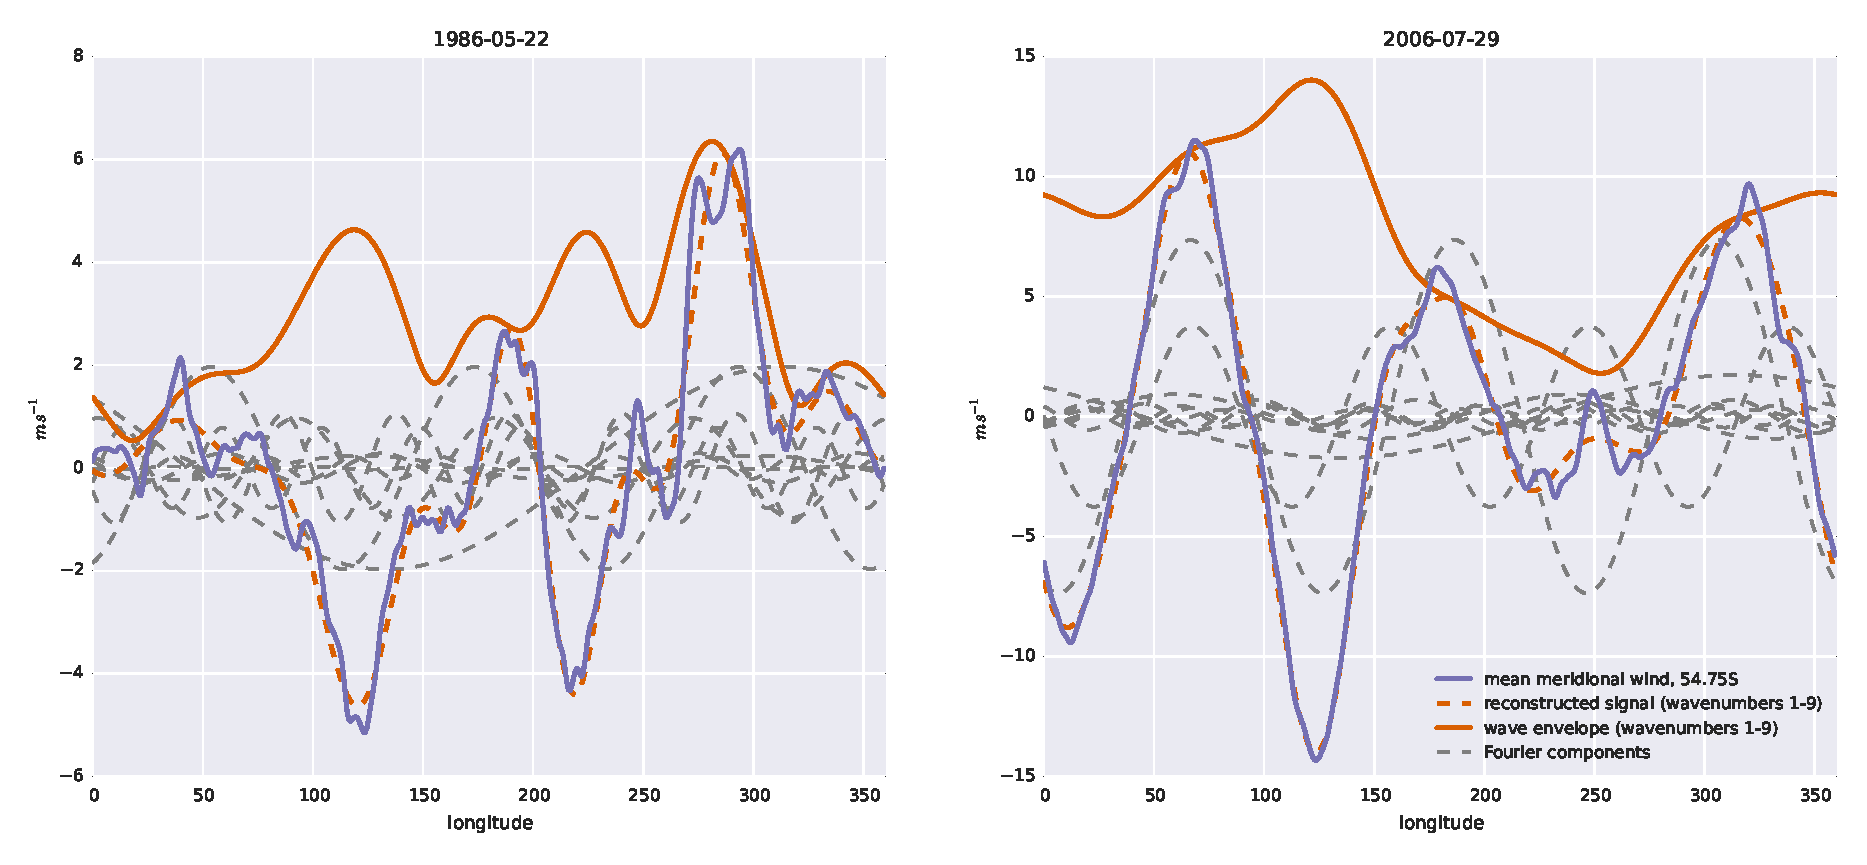
\includegraphics[width=1\columnwidth]{figures/zonalwaves/hilbert_zw_w19_va_ERAInterim_500hPa_030day-runmean_native-55S_1986-05-22_2006-07-29.eps}
\caption[Wave envelope of the 30 day running mean, 500 hPa meridional wind for 22 May 1986 and 29 July 2006 at 54.75$^{\circ}$S]{\label{fig:example_hilbert}
Wave envelope of the 30 day running mean, 500 hPa meridional wind for 22 May 1986 and 29 July 2006 at 54.75$^{\circ}$S. The original meridional wind (purple), individual Fourier components for wavenumbers 1--9 (as defined in Equation \ref{eq:fourier_transform}; grey dashed), reconstructed signal from the inverse Fourier transform (Equation \ref{eq:inverse_transform} with wavenumbers 1--9 retained; dashed orange), and wave envelope (Equation \ref{eq:wave_envelope}; solid orange) are all shown. %
}
\end{center}
\end{figure}

Subsequent studies have gone on to apply the \citet{Zimin2003} algorithm in the context of identifying and tracking Rossby wave packets in daily timescale data \citep{Glatt2014,Souders2014}, however its utility in identifying waveforms on longer temporal and larger spatial scales has not previously been investigated. In these studies, a spatial map of the wave envelope is constructed for each data time (i.e. $E(t,\lambda,\phi)$, where $t$, $\lambda$ and $\phi$ represent time, latitude and longitude respectively). The utility of these maps is evident when considering the two maps (Figure \ref{fig:example_envelope}) that correspond to the single-latitude examples shown in Figure \ref{fig:example_hilbert}. For (the diurnal averages of) both 22 May 1986 and 29 July 2006, it is clear that the wavenumber three component of the Fourier transform is dominant at 54.75$^{\circ}$S (and at the other nearby latitudes not shown in Figure \ref{fig:example_hilbert}). An analysis based on single wavenumbers could lead one to believe that both data times are associated with a pronounced hemispheric ZW3 pattern, despite the fact that this is clearly only true for 29 July (Figure \ref{fig:example_envelope}). On 22 May the spatial scale of the anomalous flow from 200 to 260$^{\circ}$E approximately matches wavenumber three, but elsewhere the flow is strongly zonal. The other components of the Fourier transform serve to modulate the wavenumber three component accordingly, and by using the wave envelope as opposed to a single wavenumber approach, this useful information is retained.

\begin{figure}
\begin{center}
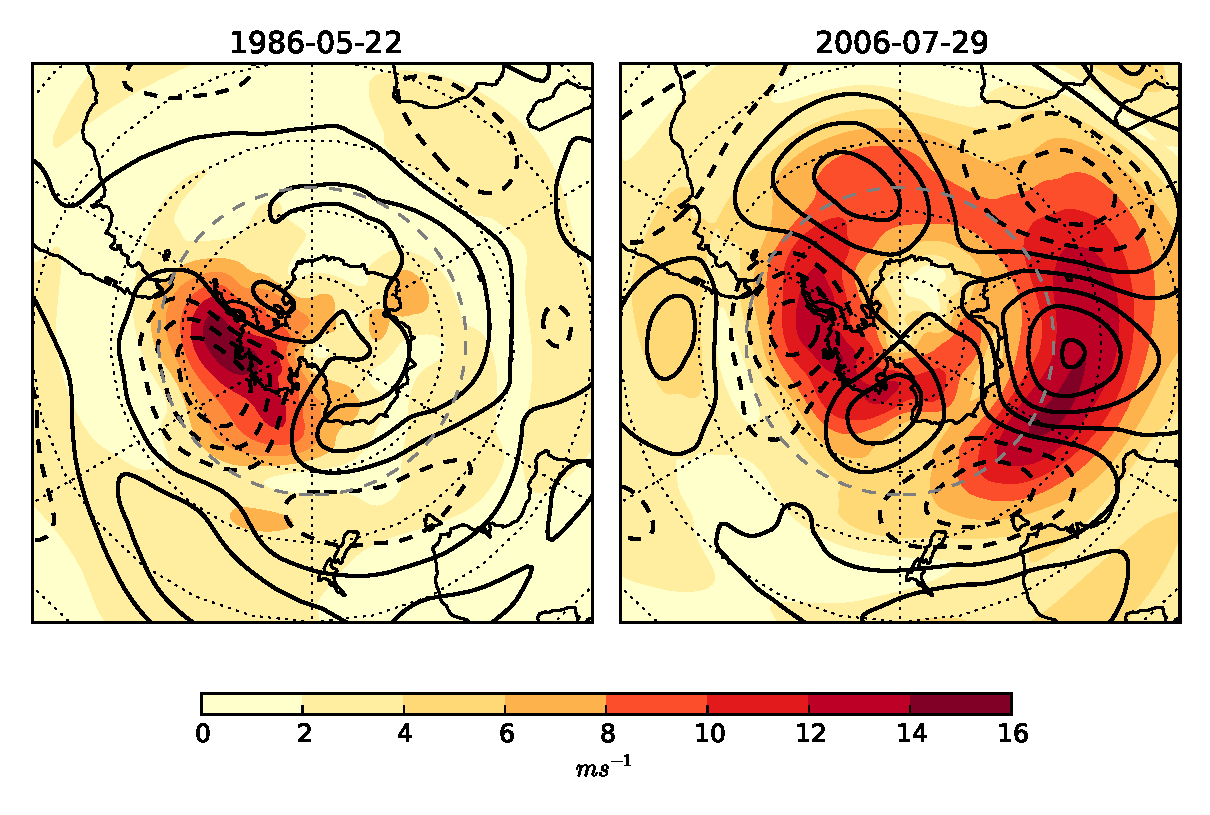
\includegraphics[width=0.84\columnwidth]{figures/zonalwaves/envva-w19_ERAInterim_500hPa_030day-runmean_native_1986-05-22_2006-07-29.eps}
\caption[Spatial wave envelope field (calculated from the 30 day running mean, 500 hPa meridional wind) for 22 May 1986 and 29 July 2006]{\label{fig:example_envelope}
Wave envelope (calculated from the 30 day running mean, 500 hPa meridional wind) for 22 May 1986 and 29 July 2006. The black contours show the corresponding 500 hPa streamfunction zonal anomaly (dashed contours indicate negative values and the contour interval is $5 \times 10^6 \: m^2 s^{-1}$). Wavenumbers 1--9 were retained and the 54.75$^{\circ}$S latitude band is indicated with a grey dashed line for ease of comparison with Figure \ref{fig:example_hilbert}. %
}
\end{center}
\end{figure}


\subsection{Index of planetary wave activity}

To define and calculate an appropriate metric of zonal (or planetary) wave activity, $E(t,\lambda,\phi)$ was calculated from the 500 hPa meridional wind. The latitudinal dimension of $E(t,\lambda,\phi)$ was eliminated by determining the meridional maximum over the range 40 to 70$^{\circ}$S, and then the zonal median was taken to eliminate the longitudinal dimension and arrive at a single `Planetary Wave Index' (PWI) value for each data time. Since wavenumbers 1--9 were retained during the process (i.e. essentially all wavenumbers), the PWI represents an integrated measure of the `waviness' of the hemispheric circulation.

The meridional wind ($v$) was used in calculating the PWI because it fundamentally reflects the presence of waves in the zonal flow. If the flow is purely zonal there are no waves and $v = 0$, while the magnitude of $v$ reflects the activity of the waves. The meridional wind is also directly involved with meridional transports of heat and moisture, which impacts directly on surface temperature, precipitation and sea ice. In fact, many studies have shown that $v$ (either filtered or unfiltered) contains much more dynamic information than alternatives such as the geopotential height ($Z$) or streamfunction \citep[e.g.][]{Berbery1996,Hoskins2005,Petoukhov2013}, neither of which has a \textit{direct} involvement with meridional exchanges. 

While better suited to the purposes of this study, the selection of $v$ has important implications for the Fourier analyses presented below. From the geostrophic relation we know that $v \propto dZ / dx$, which means that $Z$ tends to be dominated by longer wavelengths (or smaller wavenumbers) than $v$. In particular, since $Z$ is a sinusoidal function of $x$ in Fourier space, it follows that $v_k \propto k Z_k$ for any given wavenumber $k$, meaning more of the variance in $v$ is explained by shorter waves (i.e. higher wavenumbers) than it is for $Z$. This is an important distinction that is discussed further in Section \ref{s:zw_results}. Besides the selection of the meridional wind, a number of other factors were taken into consideration in devising this methodology:
\begin{itemize}
\item The results show little sensitivity to the choice of atmospheric level because the zonal waves waves are approximately equivalent barotropic. 500 hPa was selected as it represents a mid-to-upper tropospheric level that is below the tropopause in all seasons and at all latitudes of interest.
\item The wave envelope is slightly smoother if wavenumbers greater than nine are left out of the Hilbert transform, but otherwise the result is not appreciably different from when all wavenumbers are retained.
\item The meridional maximum (over 40 to 70$^{\circ}$S) was taken to allow for slight north/south variations in the mean latitude of planetary wave activity and also for the fact that the waveform is not perfectly zonally oriented. 
\item The zonal median (as opposed to the mean or integral) was taken to guard against large values in one part of the hemisphere overly influencing the end result.
\end{itemize}

      
%================================

\section{Results}\label{s:zw_results}

The results begin with a summary of the spatial and temporal characteristics of SH planetary wave activity, before considering its relationship with the major modes of SH climate variability (SAM and ENSO) and surface conditions. 

\subsection{Spatial characteristics}\label{s:zw_spatial_characteristics}

Visual inspection of the SH circulation revealed that data times of PWI greater than the 90th percentile overwhelmingly exhibit a mixed ZW1 / ZW3 hemispheric planetary wave pattern (Figure \ref{fig:pwi_spatial_summary}). Data times of PWI less than the 90th percentile become increasingly unlikely to exhibit a coordinated hemispheric wave pattern, so the 90th percentile was taken as a threshold value for planetary wave activity. 

While the coordinated, hemispheric nature of the pattern shown in Figure \ref{fig:pwi_spatial_summary} is essentially unique to data times where the PWI is greater than its 90th percentile, it is important to note that there are elements of that mixed ZW1 / ZW3 pattern that are not. In particular, it appears that the ZW1 component is relatively insensitive to changes in the strength of the meridional flow. The main difference between days of very strong (PWI $>$ 90th percentile) and very weak (PWI $<$ 10th percentile) meridional flow was instead the prominence of the ZW3 component (Figure \ref{fig:periodograms}a). While influential at all times, the ZW3 component was far more prominent when the meridional flow was strong and therefore dominated the streamfunction anomaly patterns (and thus surface impacts) discussed in analysis of surface conditions below (Section \ref{s:surface_conditions}). 

\begin{figure}
\begin{center}
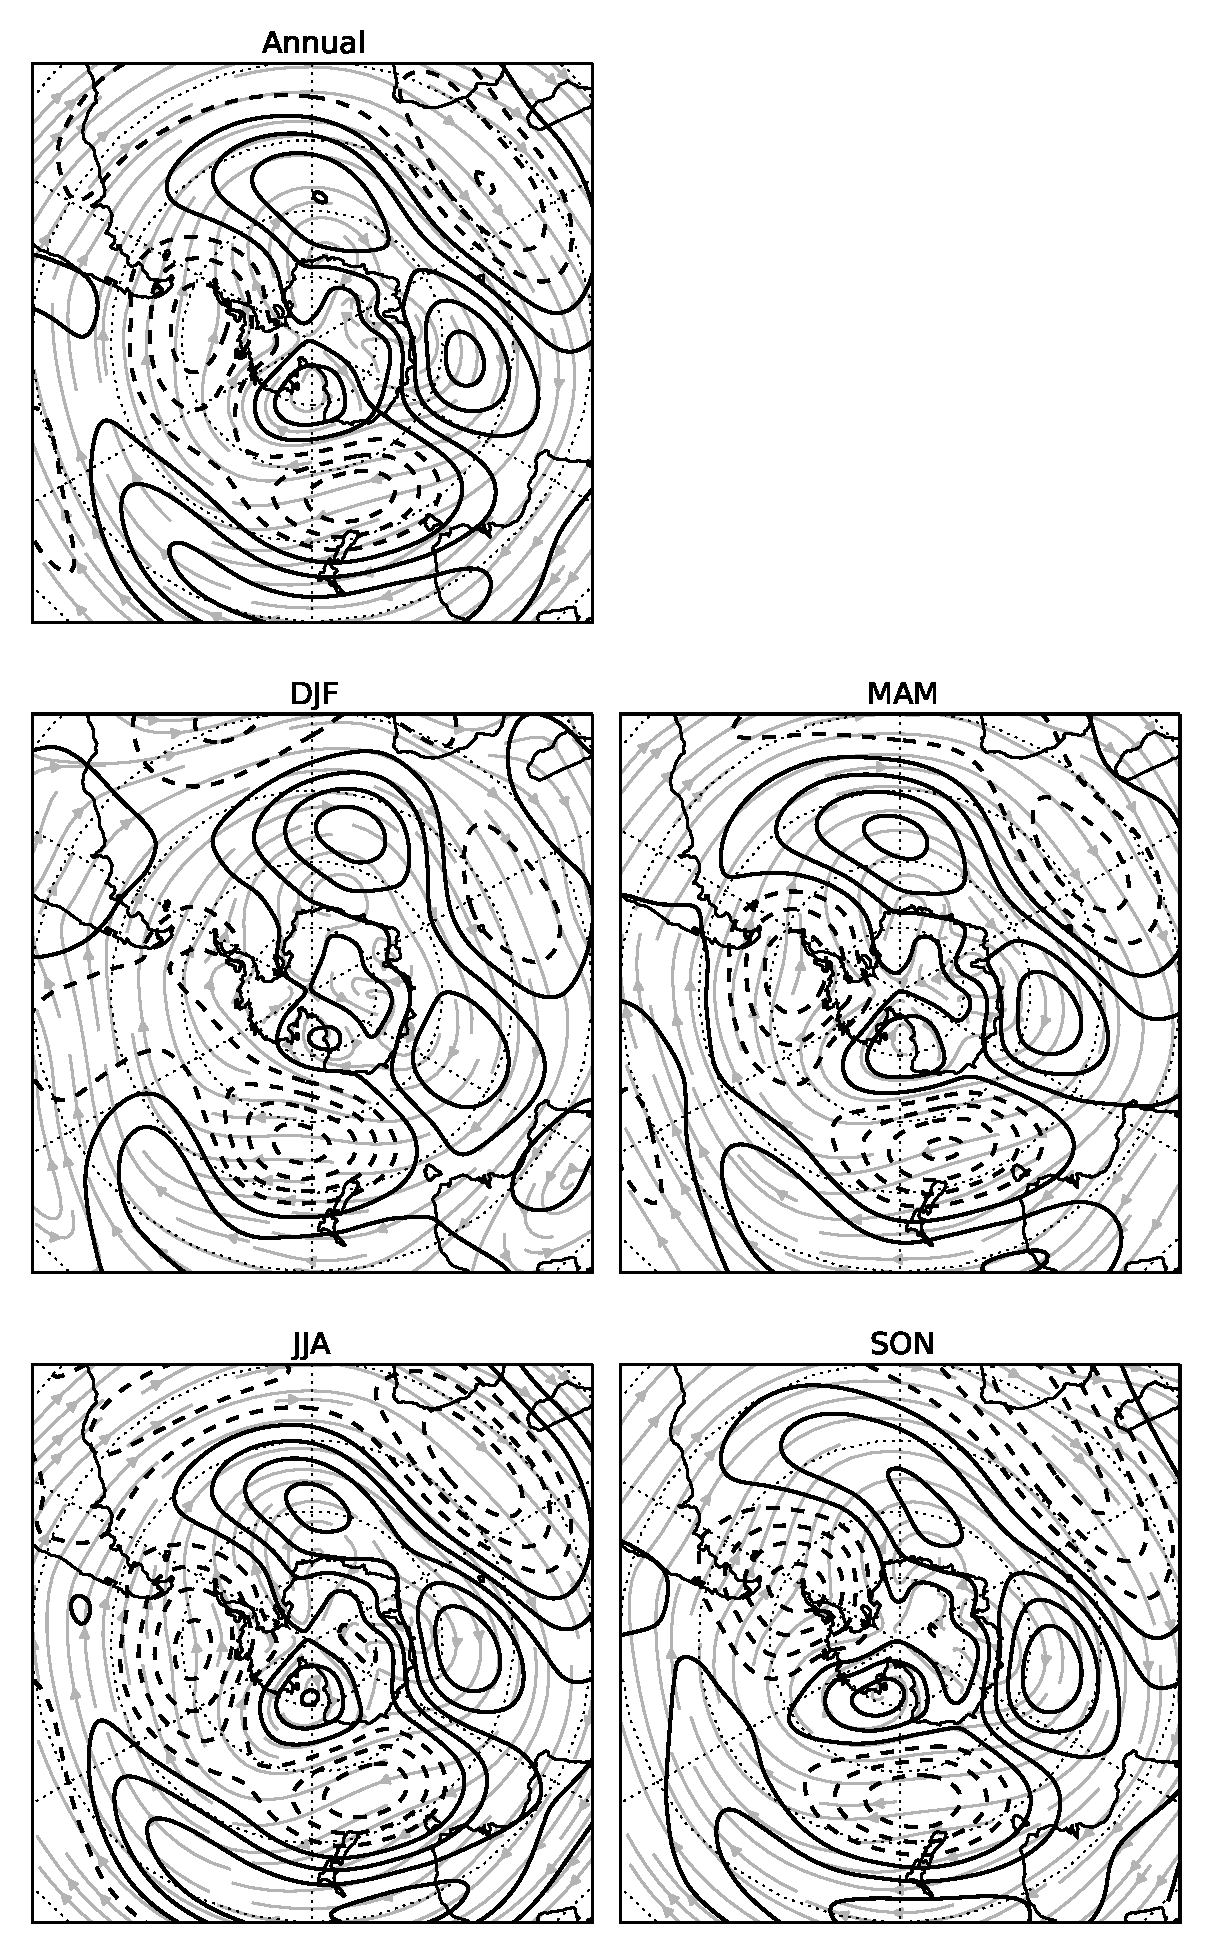
\includegraphics[width=0.7\columnwidth]{figures/zonalwaves/sf-composite_pwigt90pct_ERAInterim_500hPa_030day-runmean_native-zonal-anom-shextropics15.eps}
\caption[Composite mean 500 hPa circulation for data times where the PWI was greater than its 90th percentile]{\label{fig:pwi_spatial_summary}
Composite mean 500 hPa circulation for data times where the PWI was greater than its 90th percentile. Grey streamlines indicate the direction of the composite mean wind, while the black contours show the composite mean streamfunction zonal anomaly (dashed contours indicate negative values and the contour interval is $2.5 \times 10^6 \: m^2 s^{-1}$).}
\end{center}
\end{figure}

\begin{figure}
\begin{center}
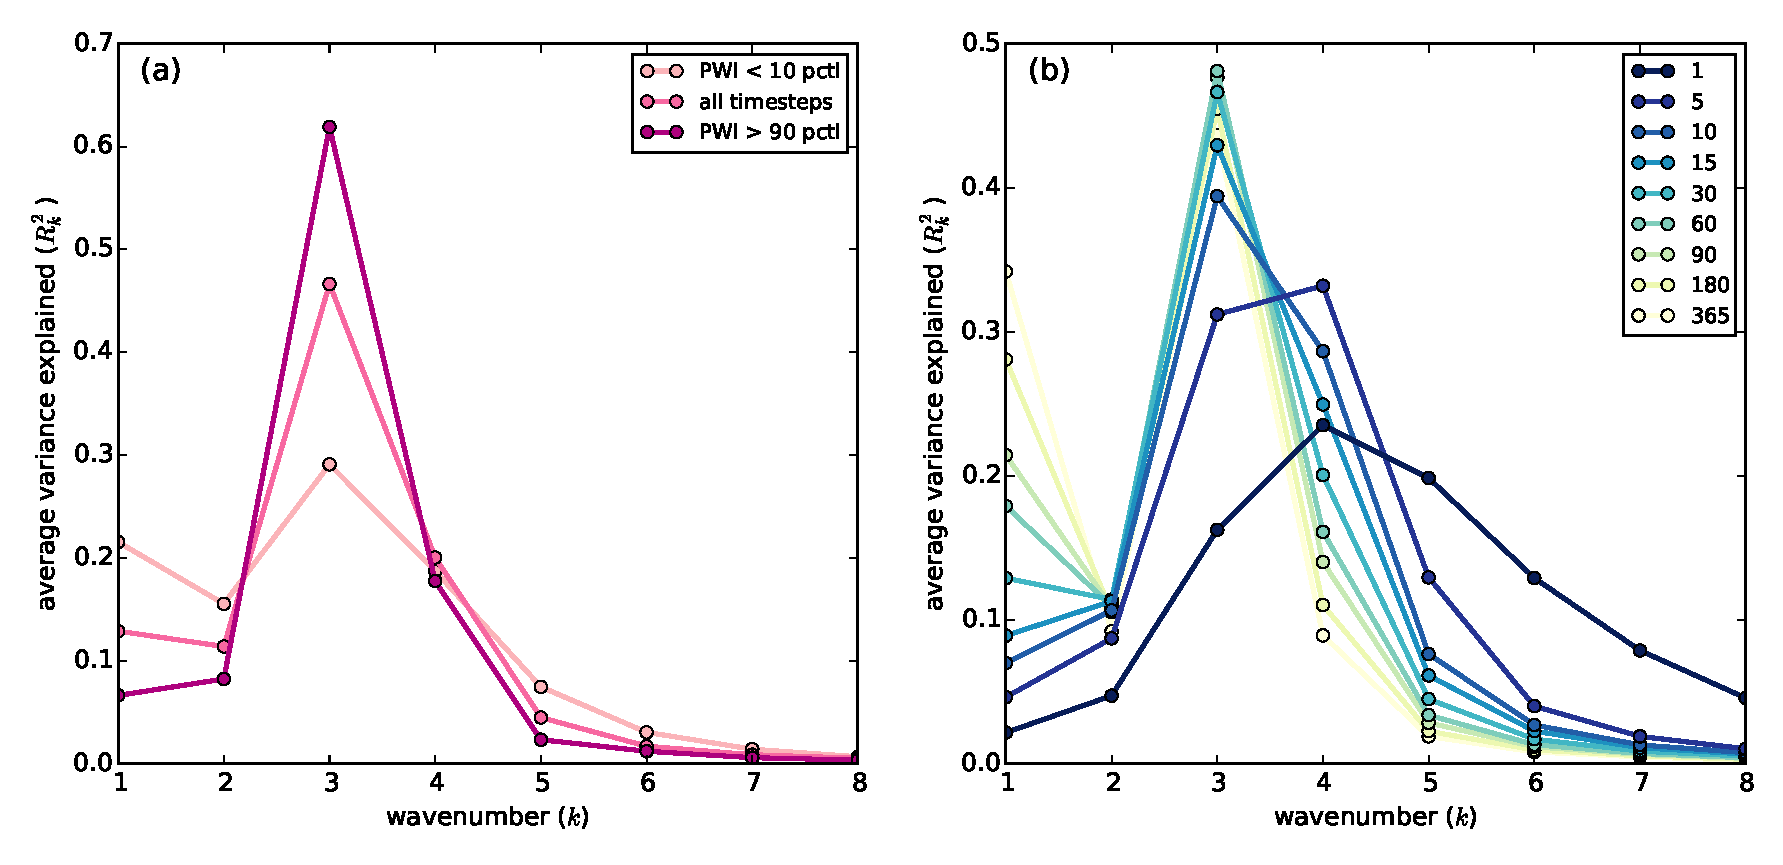
\includegraphics[width=1\columnwidth]{figures/zonalwaves/va-r2spectrum_ERAInterim_500hPa_daily_native-55S.eps}
\caption[Temporal average (1979--2014) periodograms for the 500 hPa meridional wind at 54.75$^{\circ}$S]{\label{fig:periodograms}
Temporal average (1979--2014) periodograms for the 500 hPa meridional wind at 54.75$^{\circ}$S. Panel (a) shows three different subsets of the 30 day running mean data (all data times, PWI greater than its 90th percentile, PWI less than its 10th percentile), while panel (b) includes all data times but varies the running mean (in days) applied to the data prior to the Fourier transform. The labels on the vertical axis correspond to Equation \ref{eq:variance_explained}.}
\end{center}
\end{figure}


Given the dominance of the ZW3, it is not surprising that the ZW3 index of \citet{Raphael2004} shows a reasonably high level of agreement with the PWI (Figure \ref{fig:metric_vs_zw3}). Having said that, it is important to note that the shading of the dots in Figure \ref{fig:metric_vs_zw3} --- which represent the phase of the wavenumber three component of the Fourier transform --- are not randomly distributed. Whenever the phase of the wavenumber three component of the flow does not match up with the location of the three grid points used to calculate the ZW3 index (indicated by the dark red or near-white shading in Figure \ref{fig:metric_vs_zw3}), a low value is recorded for the ZW3 index. The outlying dots in the bottom right hand quadrant are particularly noteworthy, as in these cases the PWI (and hence in most cases the amplitude of the wavenumber three component of the flow) is actually quite large. The failure of the ZW3 index to capture these out-of-phase patterns means that composite analyses based on that index may overstate the stationarity (and hence the time-mean impacts) of the ZW3 component of the flow.

\begin{figure}
\begin{center}
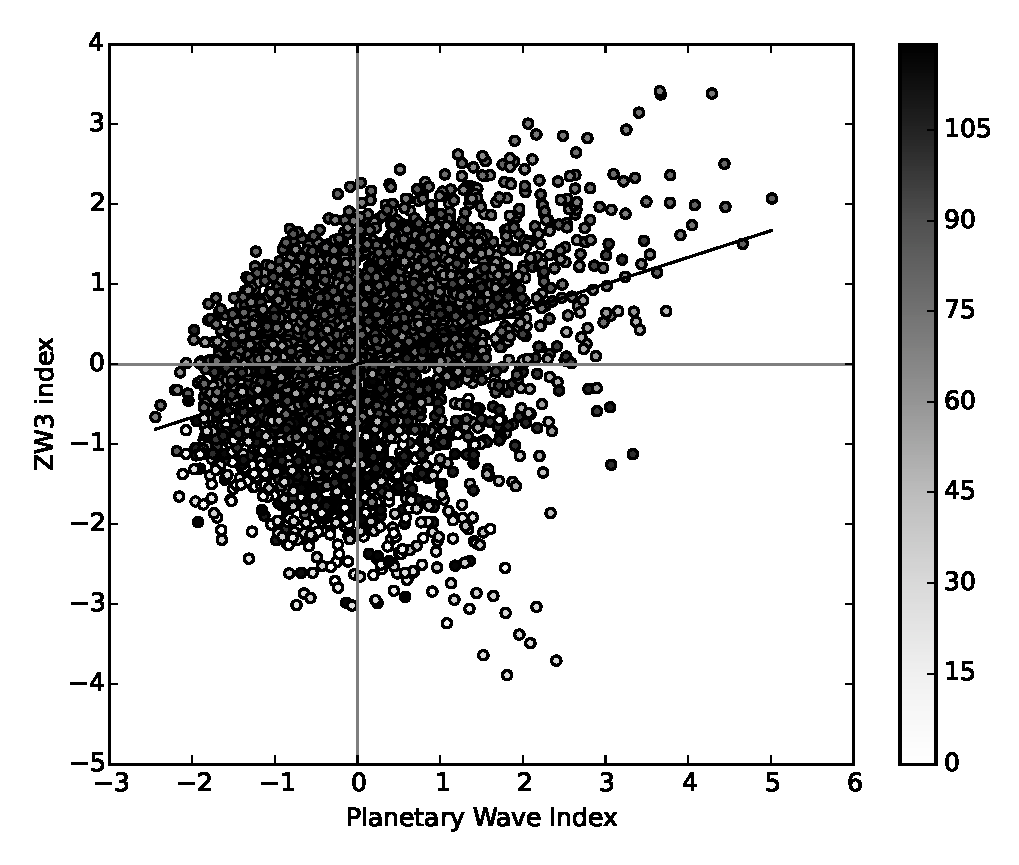
\includegraphics[width=0.8\columnwidth]{figures/zonalwaves/pwi-vs-zw3index_ERAInterim_500hPa_030day-runmean_native.eps}
\caption[PWI versus the ZW3 index of \citet{Raphael2004}]{\label{fig:metric_vs_zw3}
PWI versus the ZW3 index of \citet{Raphael2004}. Both were calculated using 500 hPa, 30 day running mean data (the PWI was calculated from the meridional wind and the ZW3 index from the geopotential height zonal anomaly). The shading represents the phase of the wavenumber three component of the Fourier transform of the meridional wind (expressed as the location, in degrees east, of the first local maxima), while the black line is a linear least-squares line of best fit. Both indices have been normalised to aid visual comparison (for each index this involved subtracting the mean of the index series and then dividing by the standard deviation).}
\end{center}
\end{figure}
    
\subsection{Temporal characteristics}

Consistent with previous studies \citep[e.g.][]{vanLoon1984,Mo1985}, the composite mean 500 hPa streamfunction zonal anomaly pattern for data times where the PWI exceeds its 90th percentile (Figure \ref{fig:pwi_spatial_summary}) migrates zonally by approximately 15$^{\circ}$ from its most easterly location during summer to its most westerly during winter (notwithstanding the fact that the pattern breaks down from around 240 to 330$^{\circ}$E during summer). It has a slightly larger amplitude during the winter months and the frequency of strong planetary wave activity was also far more pronounced at that time of the year (Figure \ref{fig:annual_distribution}b). The seasonal counts of the number of data times exceeding the PWI 90th percentile (Figure \ref{fig:annual_distribution}a) show that 1980 was associated with a particularly high frequency of planetary wave activity, however there were no statistically significant linear trends in these counts for timeseries including (Figure \ref{fig:annual_distribution}c) or excluding (i.e. 1981--2014) the year 1980.  

\begin{figure}
\begin{center}
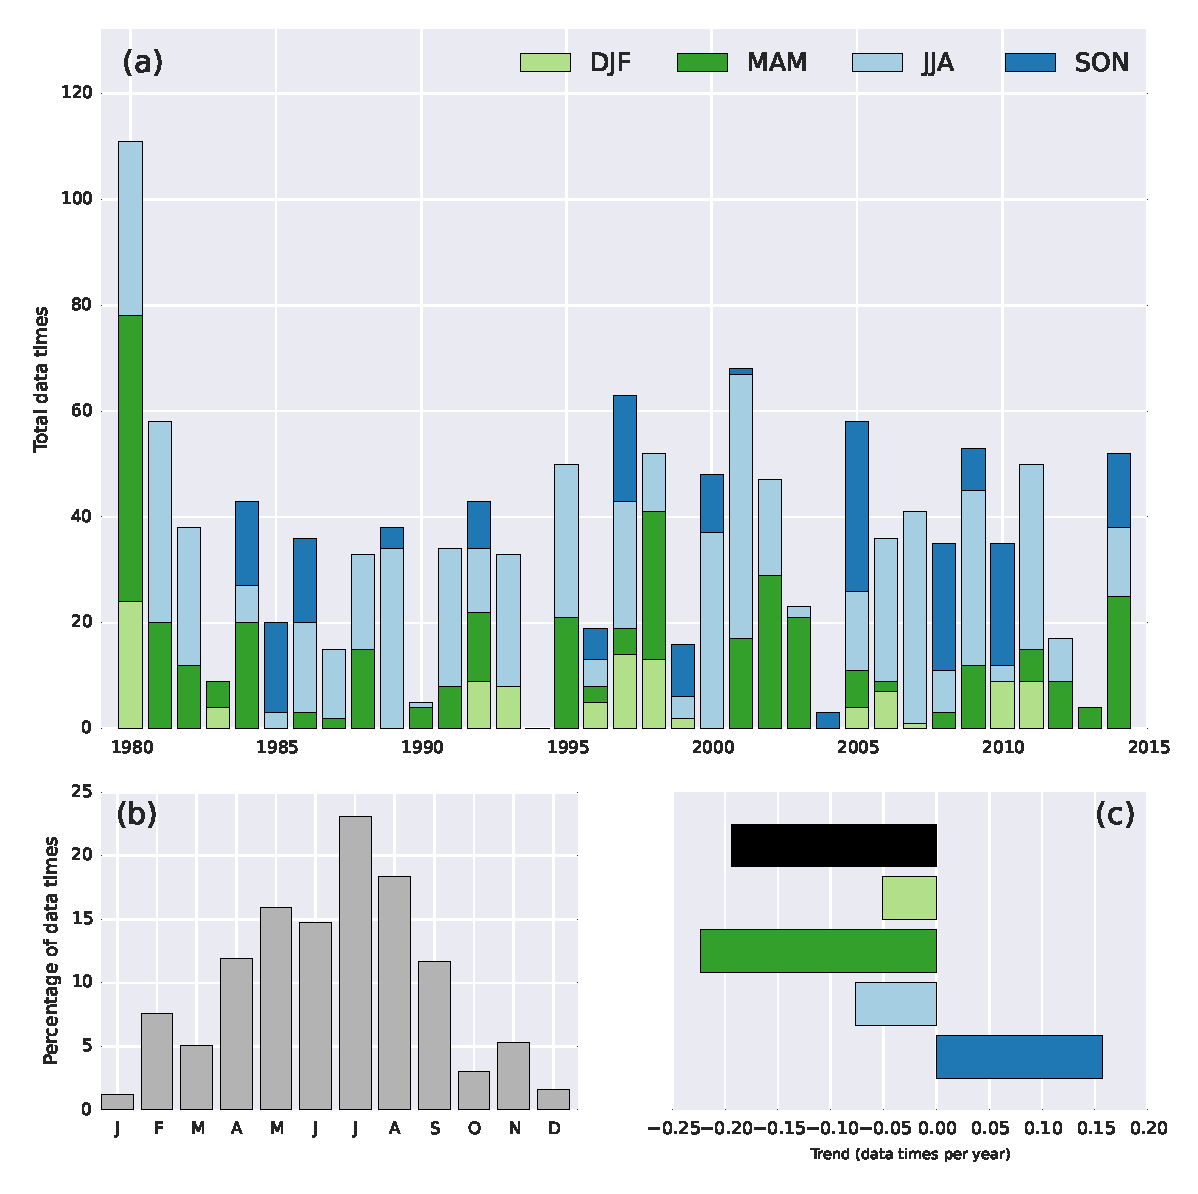
\includegraphics[width=0.7\columnwidth]{figures/zonalwaves/dates-summary_pwigt90pct_ERAInterim_500hPa_030day-runmean_native.eps}
\caption[Variability and trends in data times where the PWI was greater than its 90th percentile]{\label{fig:annual_distribution}
Variability and trends in data times where the PWI was greater than its 90th percentile. The total data times for each individual season are shown in panel (a), corresponding seasonal linear trends in panel (c) (black represents the annual trend) and monthly totals for the entire study period (1979--2014) in panel (b). To account for the fact that not all months have an equal number of days, the counts for each month in panel (b) are presented as a percentage of the total number of days for that month. Years in panel (a) are defined from December to November (e.g. the `year' 1980 spans December 1979 to November 1980) and none of the trends shown in panel (c) are statistically significant at the $p < 0.10$ level.}
\end{center}
\end{figure}

While the results presented here focus is on the monthly (30 day running mean) timescale, it is interesting to consider whether similar behaviour is observed at other timescales. It can be seen from Figure \ref{fig:periodograms}b that wavenumber three dominates the average periodogram when the running mean applied to the daily 500 hPa meridional wind is greater than 10 days, with wavenumber one becoming progressively more influential as the smoothing increases. When the same process is repeated using the 500 hPa geopotential height (not shown), the results are very different. The ZW1 dominates at all timescales and except for a slight upswing from wavenumber two to three, the variance explained monotonically decreases for subsequent wavenumbers. This is an important result because \citet{vanLoon1972} analysed geopotential height data and concluded that ZW1 explains (by an appreciable margin) the largest fraction of the spatial variance in the 500 hPa SH circulation (a finding that has been quoted in many subsequent papers). In light of the results presented here and the previous discussion concerning the fact that $v_k \propto k Z_k$ in Fourier space and that the meridional wind may be a more appropriate quantity to analyse in this context, it is clear that ZW3 plays a greater role than previously thought, particularly when there is a strong meridional component to the hemispheric flow. 

  
\subsection{SAM and ENSO}

Composite analysis was also used to assess the relationship between the PWI and the major modes of SH climate variability. SAM events were defined according to the 75th and 25th percentiles of the AOI, while positive (El Ni\~{n}o) and negative (La Ni\~{n}a) ENSO events were defined as a Ni\~{n}o 3.4 above 0.5$^{\circ}$C and below -0.5$^{\circ}$C respectively. Composites for each phase of SAM and ENSO were then calculated by taking the average across all data times for which the PWI exceeded its 90th percentile \textit{and} the AOI or Ni\~{n}o 3.4 was greater or less than the relevant threshold. 

The SAM composites show that the phase of the planetary wave pattern moves east during positive SAM events and west during negative events (Figure \ref{fig:sam_composite}). Planetary wave activity was also more common when the SAM was negative: of the 1312 data times where the PWI exceeded its 90th percentile, 510 (39\%) had an AOI that was less than the 25th percentile as compared to only 166 (13\%) with an AOI greater than the 75th percentile. Consistent with this finding, the aforementioned outlying year for planetary wave activity (1980; see Figure \ref{fig:annual_distribution}b) was associated with a large negative SAM.

The association between ENSO and planetary wave activity was far less pronounced. Besides a subtle east (La Ni\~{n}a) / west (El Ni\~{n}o) movement of the anticyclone over the south-east Pacific, no appreciable changes were seen in the phase of the planetary wave pattern (not shown) and planetary wave activity was only slightly more common during El Ni\~{n}o conditions (282 data times to 176).      

\begin{figure}
\begin{center}
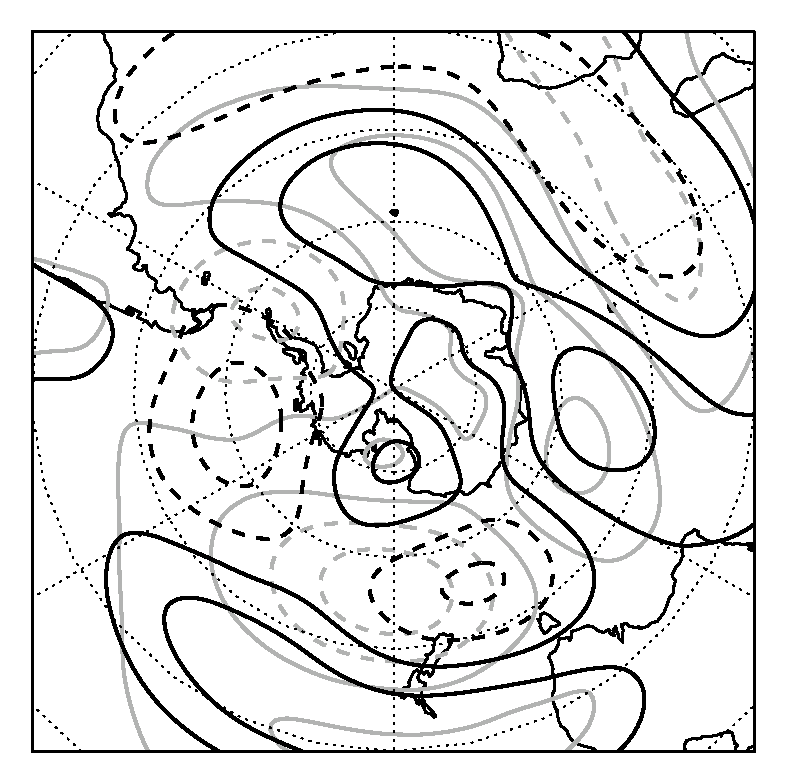
\includegraphics[width=0.56\columnwidth]{figures/zonalwaves/sf-composite_samgt75pct-samlt25pct-pwigt90pct_ERAInterim_500hPa_030day-runmean_native-zonal-anom-shextropics15.eps}
\caption[Comparison of the composite mean 500 hPa streamfunction zonal anomaly for data times where the PWI was greater than its 90th percentile and the SAM was (a) positive and (b) negative]{\label{fig:sam_composite}
Composite mean 500 hPa streamfunction zonal anomaly for data times where the PWI was greater than its 90th percentile \textit{and} the AOI was greater than its 75th percentile (grey) or less than its 25th percentile (black). Dashed contours indicate negative values and the contour interval is $4.0 \times 10^6 \: m^2 s^{-1}$.}
\end{center}
\end{figure}


\subsection{Surface conditions}\label{s:surface_conditions}

In order to assess the influence of planetary wave activity on regional climate variability, composite means of variables of interest (the surface air temperature anomaly, precipitation anomaly and sea ice concentration anomaly) were calculated for all data times where the PWI exceeded its 90th percentile. In other words, the analysis posed the question: what is the average temperature (or precipitation or sea ice concentration) anomaly when there is strong planetary wave activity? The anomalous flow associated with these composites (indicated by the 500 hPa streamfunction anomaly as opposed to the streamfunction \textit{zonal} anomaly shown earlier) has a very strong ZW3 signature. This is consistent with the spatial characteristics presented earlier (Section \ref{s:zw_spatial_characteristics}), which indicate that the distinguishing feature of data times of strong meridional flow is the enhanced ZW3 component (as opposed to ZW1).  


\subsubsection{Surface air temperature}

Planetary wave activity was found to be associated with large and widespread surface air temperature anomalies over and/or around much of West Antarctica during all seasons (Figure \ref{fig:tas_composite}). The most pronounced anomalies were seen during autumn and winter, with warmer than average conditions over the interior of West Antarctica (associated with an anomalous northerly flow) and correspondingly colder than average conditions over the Weddell Sea (associated with an anomalous southerly flow). Due to the aforementioned seasonal migration (and breakdown during summer) of the mean planetary wave pattern, warm anomalies were confined to the Antarctica Peninsula during spring, while summer was associated with the smallest anomalies of any season.  

With respect to other sectors of the high southern latitudes, anomalously warm temperatures were widespread over East Antarctica during all seasons except summer. The largest anomalies were seen over Wilkes Land during autumn and winter, in association with an anomalous northerly flow in that region. Other features of note included anomalously cool temperatures over the Ross Sea and mainland Australia during spring.

\begin{figure}
\begin{center}
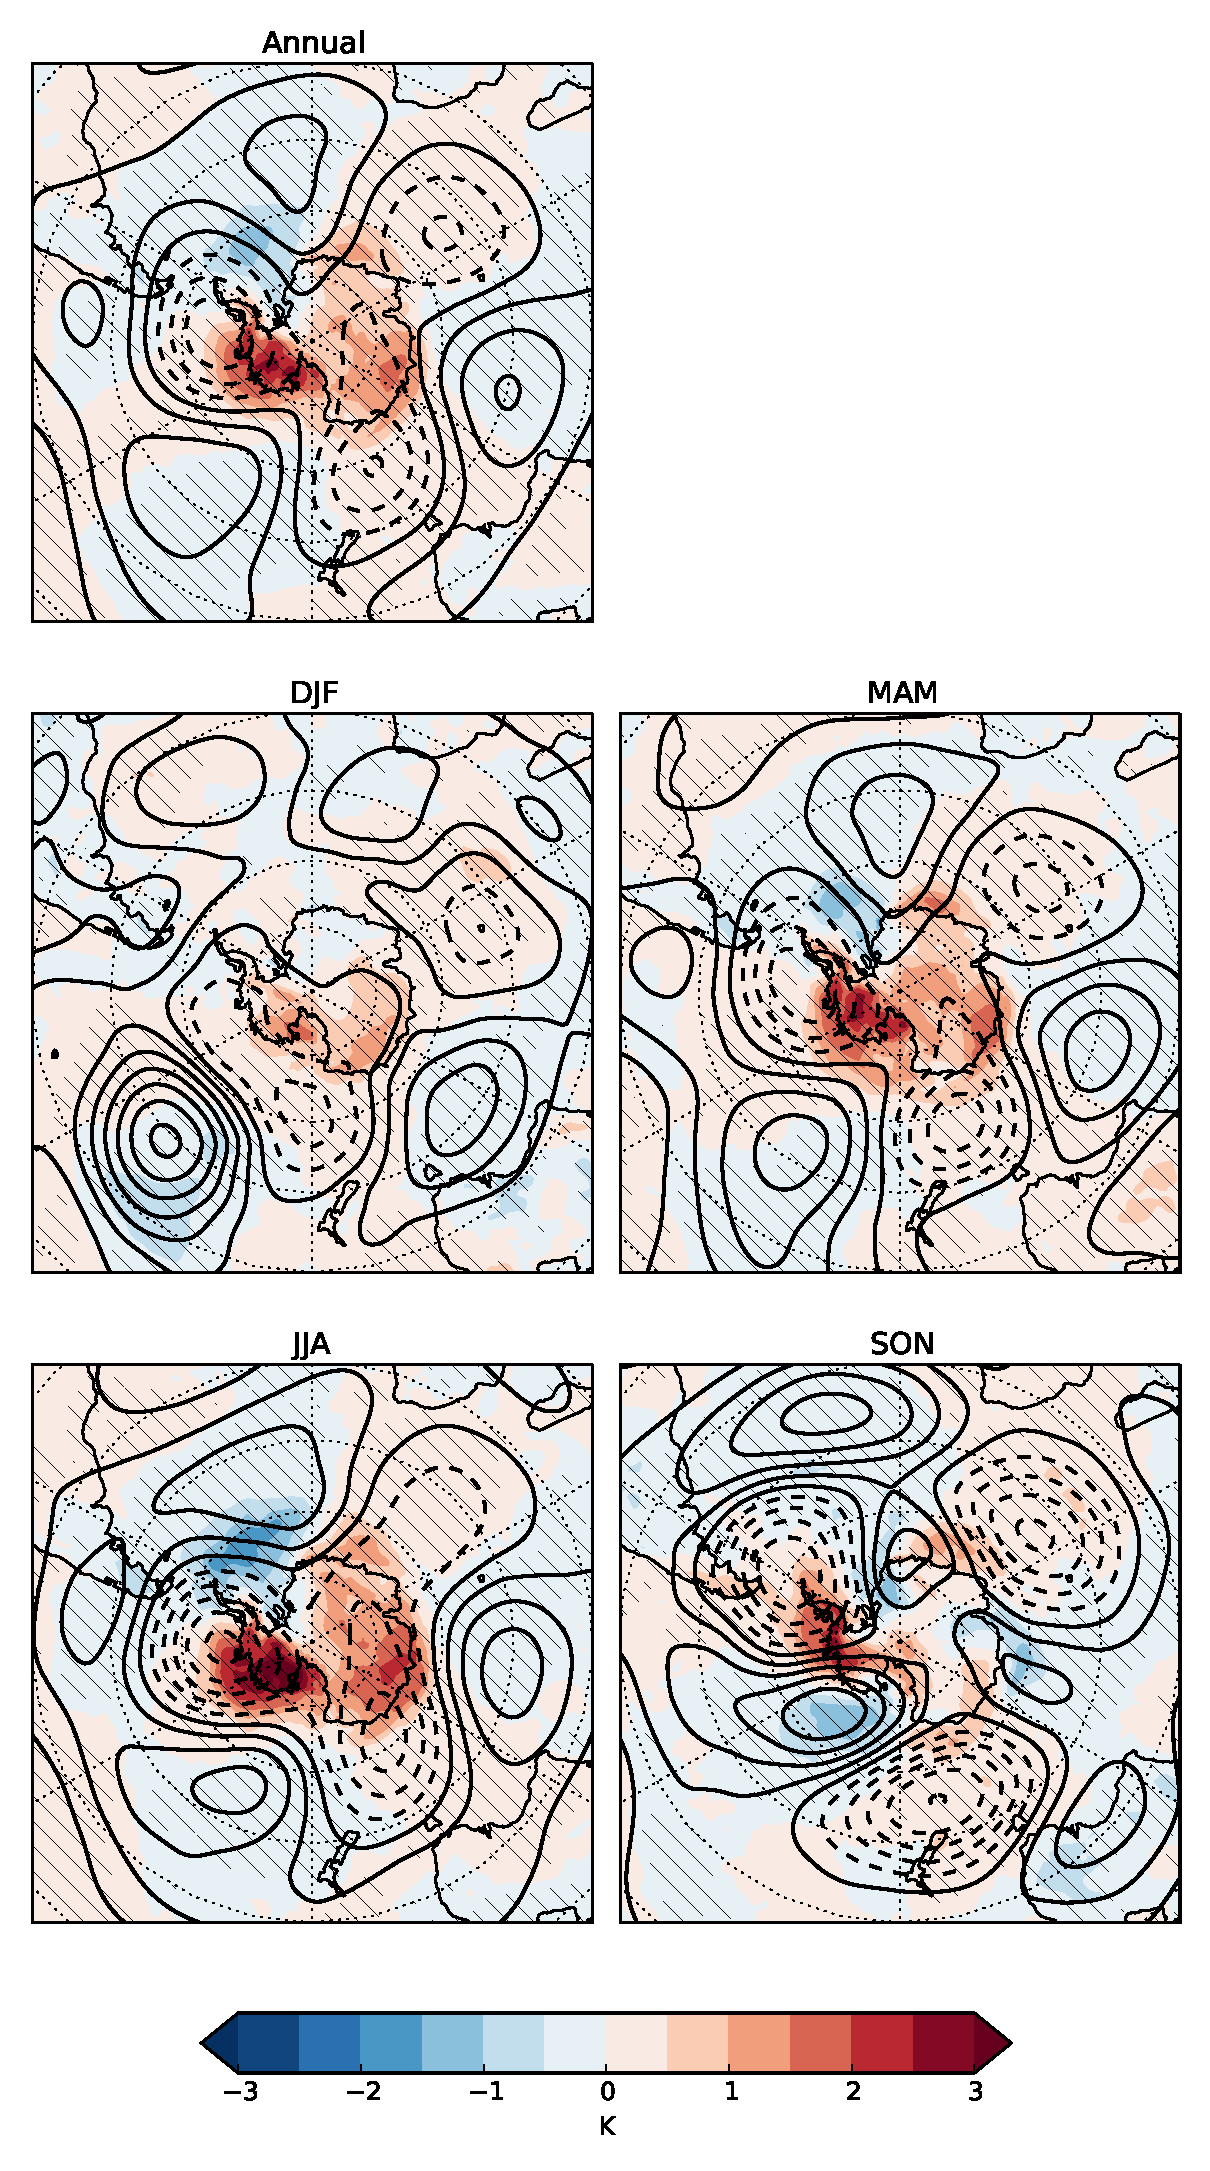
\includegraphics[width=0.63\columnwidth]{figures/zonalwaves/tas-composite_pwigt90pct_ERAInterim_500hPa_030day-runmean-anom-wrt-all_native-shextropics15.eps}
\caption[Composite mean surface air temperature anomaly for data times where the PWI was greater than its 90th percentile]{\label{fig:tas_composite}
Composite mean surface air temperature anomaly for data times where the PWI was greater than its 90th percentile. Black contours show the corresponding composite mean 500 hPa streamfunction anomaly (dashed contours indicate negative values and the contour interval is $2.5 \times 10^6 \: m^2 s^{-1}$), while the hatching shows regions where the difference between the composite mean and climatological mean is significant at the $p < 0.01$ level.}
\end{center}
\end{figure} 

\subsubsection{Precipitation}

The seasonal composite mean precipitation anomalies generally displayed an alternating wet/dry pattern of wavenumber three, consistent with the upper level low/high pressure anomalies associated with the enhanced ZW3 component of the hemispheric circulation. Within this pattern, the largest anomalies corresponded to regions of either enhanced or suppressed flow over significant topography (Figure \ref{fig:pr_composite}). For instance, the same anomalous onshore flow that was associated with high temperatures over both West Antarctica and Wilkes Land was also associated with large positive coastal precipitation anomalies, with the precise location of those anomalies moving with seasonal variations in the location of the mean planetary wave pattern. In contrast, weakened westerly flow over the southern Andes during autumn, winter and spring (but not summer due to the breakdown of the wave pattern in that region) was associated with large negative precipitation anomalies over Chilean Patagonia. A similar mechanism explains the large negative anomalies over New Zealand during winter and spring, when the mean planetary wave pattern is located sufficiently far to the west to exert an appreciable influence on the westerly flow over the South Island. Enhanced orographic precipitation due to anomalous onshore flow might also play a role in the large positive precipitation anomalies seen over eastern Australia during spring, however the anomalies extend far beyond the Great Dividing Range, suggesting that enhanced moisture transport from the Tasman Sea might be the dominant mechanism. 

\begin{figure}
\begin{center}
\includegraphics[width=0.63\columnwidth]{figures/zonalwaves/pr-composite_pwigt90pct_ERAInterim_500hPa_030day-runmean-anom-wrt-all_native-shextropics15.eps}
\caption[As per Figure \ref{fig:tas_composite}, but for the precipitation anomaly]{\label{fig:pr_composite}
As per Figure \ref{fig:tas_composite}, but for the precipitation anomaly.}
\end{center}
\end{figure}


\subsubsection{Sea ice}

The sea ice composites (Figure \ref{fig:sic_composite}) were highly consistent with the temperature composites. For instance, in autumn and winter anomalous onshore flow and warmth over the interior of West Antarctica was in accord with the reduced sea ice concentration over the Amundsen Sea, and anomalous offshore flow and cold conditions over the Weddell Sea during autumn was consistent with the increased sea ice concentration. In spring, the anomalous warmth over the western aspect of the Antarctic Peninsula concurred with the reduced sea ice concentration in the Bellingshausen Sea, while the anomalously cold temperatures over the Ross Sea coincided with an anomalously high sea ice concentration. The anomalous onshore winds and warmth over Wilkes Land were consistent with the reduced sea ice seen immediately to the north of George V Land, Ad{\'e}lie Land and the Sabrina Coast of East Antarctica in all seasons except summer (when there is very little ice there anyway). One regional feature that does not appear to fit with this overall consistency was the anomalously high sea ice concentration to the west of the Antarctic Peninsula during autumn, which was not reflected in the corresponding temperature composite.
 
\begin{figure}
\begin{center}
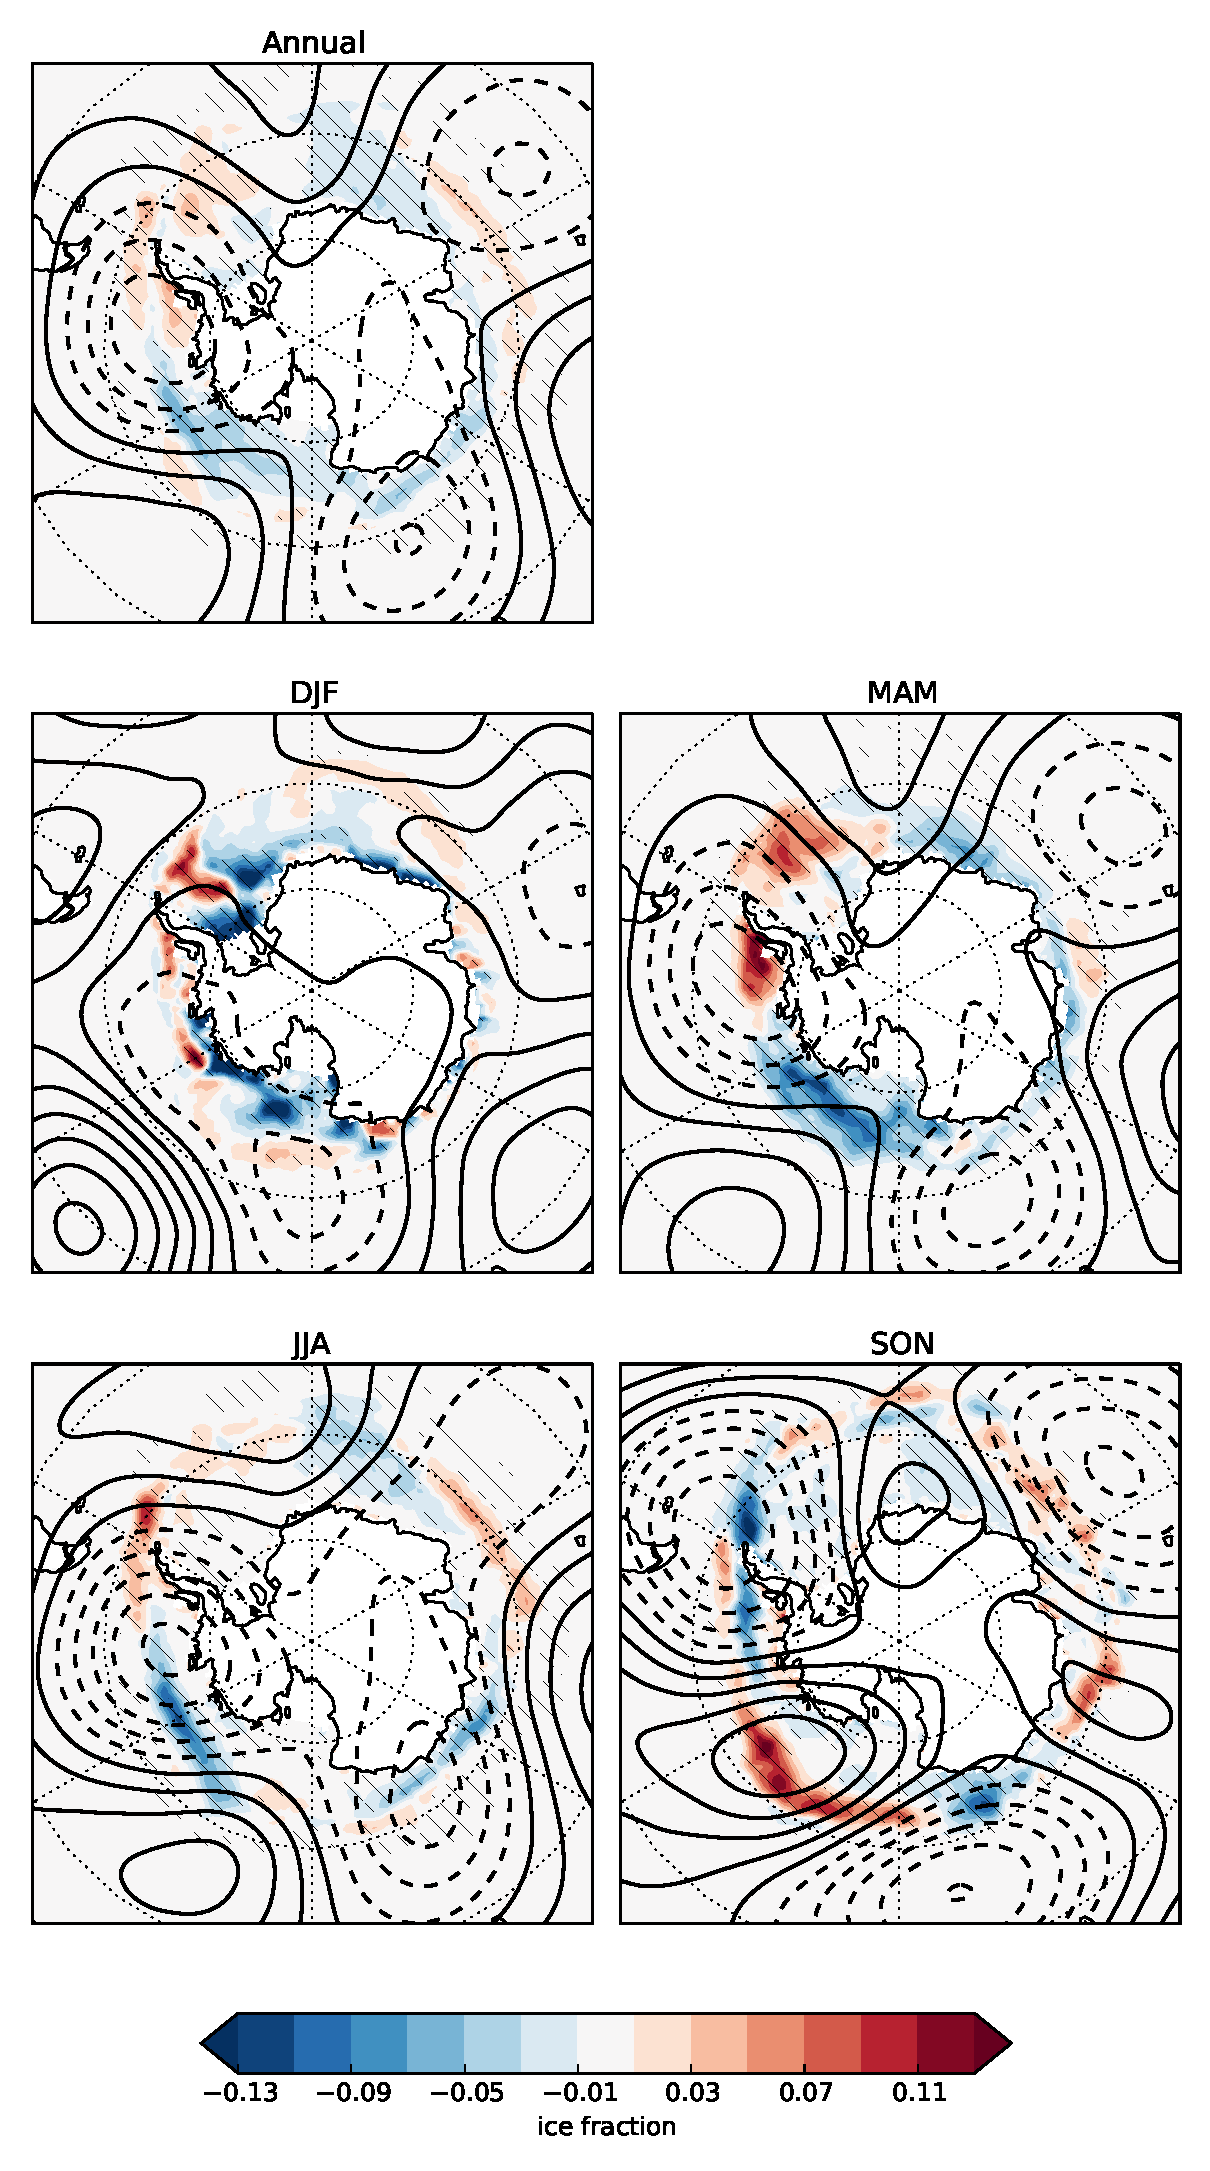
\includegraphics[width=0.63\columnwidth]{figures/zonalwaves/sic-composite_pwigt90pct_ERAInterim_500hPa_030day-runmean-anom-wrt-all_native-shextropics15.eps}
\caption[As per Figure \ref{fig:tas_composite}, but for the sea ice concentration anomaly]{\label{fig:sic_composite}
As per Figure \ref{fig:tas_composite}, but for the sea ice concentration anomaly.}
\end{center}
\end{figure}    
 

\section{Discussion}

%================================

A novel method for identifying quasi-stationary planetary wave activity has been developed and applied to the problem of characterising the SH zonal waves and their influence on regional climate variability. The method adapts the wave envelope construct traditionally used in the identification of synoptic-scale Rossby wave packets and improves on existing methods by allowing for variations in both wave phase and amplitude. The zonal wave analysis reveals that while both ZW1 and ZW3 are prominent features of the climatological SH circulation, the defining feature of highly meridional hemispheric states is an enhancement of the ZW3 component. These enhanced ZW3 states are associated with large sea ice anomalies over the Amundsen and Bellingshausen Seas and along much of the East Antarctic coastline, large precipitation anomalies in regions of significant topography and anomalously warm temperatures over much of the Antarctic continent. 

In interpreting the results, it is important to clearly define what is meant by the phrase `quasi-stationary planetary wave activity' in this context. It was evident from the analysis of the monthly timescale (30 day running mean) meridional wind that the ZW1 and ZW3 patterns are a prominent feature of the SH circulation even when the hemispheric meridional flow is weak (Figure \ref{fig:periodograms}a). As the meridional flow gets stronger the ZW3 component becomes increasingly prominent, while the ZW1 component remains relatively unchanged. This means the average anomalous flow associated with a highly meridional hemispheric state clearly resembles a ZW3 pattern (Figures \ref{fig:tas_composite}, \ref{fig:pr_composite} and \ref{fig:sic_composite}). It is this highly meridional and anomalous ZW3 circulation that is captured by high values of the PWI and thus is referred to as planetary wave activity, as opposed to the mixed ZW1 / ZW3 pattern that is essentially present at all times.  

The climatology of planetary wave activity confirms previous results regarding the seasonality of the zonal waves (peak activity in winter, seasonal migration of the zonal location/phase), and also identifies a large sector of the western hemisphere (120 to 30$^{\circ}$W) where the mean wave activity breaks down during summer. In contrast to the results presented here, previous studies have suggested a link between planetary wave activity and ENSO \citep[e.g.][]{Trenberth1980,Raphael2003,Hobbs2007}. Given the hemispheric nature of the PWI (i.e. it responds most strongly to coordinated, hemispheric patterns of meridional flow) it is perhaps not surprising that there was not a strong link with ENSO, given that teleconnections between ENSO and the high southern latitudes tend to be localised around the south-east Pacific \citep{Simmonds1995,Turner2004}. While this result is not good news for the predictability of planetary wave activity, its increased frequency during negative SAM events offers some hope. The identified east/west migration of the mean planetary wave pattern with positive/negative phases of the SAM possibly ties in with the zonally asymmetric properties of the SAM \citep[e.g.][]{Kidson1988,Kidston2009}, however a detailed analysis of this relationship was beyond the scope of this thesis.

With respect to the link between planetary wave activity and regional climate variability, most relevant investigations have focused on sea ice. The recent study of \citet{Raphael2014} takes a new approach to assessing the influence of the atmospheric circulation, focusing on the ice advance (approximately March-August) and retreat (September-February) seasons for five distinct regions of sea ice variability around Antarctica. Their examination of the spatial pattern of correlation between sea ice extent and 500 hPa geopotential height for each season/region suggests that the ZW3 pattern is the primary driver of sea ice variability in the Weddell and Amundsen/Bellingshausen Seas during the advance season. The results presented here tend to support this finding, particularly during the early part (MAM) of the advance season. In contrast, the strong association identified between the PWI and sea ice coverage just to the north of George V Land, Ad{\'e}lie Land and the Sabrina Coast in East Antarctica does not seem to be in agreement with the results of \citet{Raphael2014}, who found the SAM to be the major driver in that region for both the advance and retreat seasons.

For the King Haakon VII Sea (10$^{\circ}$W to 70$^{\circ}$E), \citet{Raphael2014} were unable to identify an obvious atmospheric driver. The results presented here suggest that planetary wave activity may play an important role there, since the correlation patterns identified by \citet{Raphael2014} bear some resemblance to the mean planetary wave patterns shown in this study. The reason the resemblance is not stronger may be due to the fact that the association between the PWI and sea ice coverage appears to be unidirectional in that region. In MAM, JJA and SON, PWI values greater than the 90th percentile are associated with anomalously low sea ice concentrations, while values less than the 10th percentile are associated with near average (as opposed to anomalously high) concentrations (not shown). Of course, any discussion of the atmospheric drivers of sea ice variability is complicated by the relationships between those drivers. For instance, the SAM and ENSO show many similarities in their influence on sea ice. It is unclear whether this is because they operate together in their response mechanism, or if the similarity is due to a preferred hemispheric planetary wave response \citep[e.g.][]{Pezza2012}. 

In contrast to the sea ice literature, planetary wave activity is scarcely mentioned in relation to SH precipitation variability, even in the regions of significant topography so clearly identified in this study. Instead, analyses of precipitation variability over New Zealand, Patagonia and eastern Australia tend to focus on the SAM and ENSO, with the former generally becoming increasingly influential at higher latitudes \citep[e.g.][]{Ummenhofer2007,Aravena2009,Kidston2009,Risbey2009,Garreaud2013,Jiang2013}. Such analyses may inadvertently capture some of the zonal wave influence due to its similarity with the zonally asymmetric features of the SAM, however \citet{Garreaud2013} do note that winter precipitation anomalies over Patagonia are dominated by a wavenumber three mode rather than a more zonally symmetric SAM pattern. Planetary wave activity also receives scant attention in overviews and analyses of Antarctic temperature variability \citep[e.g.][]{Russell2010,SchneiderOkumura2012,Yu2012}. In the main, the results presented here show that the enhanced meridional flow associated with planetary wave activity brings warm air poleward and thus large positive temperature anomalies are seen throughout most of Antarctica, particularly during autumn and winter. 
